% !TeX program = lualatex -synctex=1 -interaction=nonstopmode --shell-escape %.tex
\documentclass[beamer,xcolor=dvipsnames]{standalone}
\RequirePackage[rus]{borochkin_tikz}

\newcolumntype{C}[1]{>{\centering\arraybackslash}p{#1}}
\newcolumntype{L}[1]{>{\raggedright\arraybackslash}p{#1}}

\begin{document}
\begin{standaloneframe}[shrink=0, fragile]
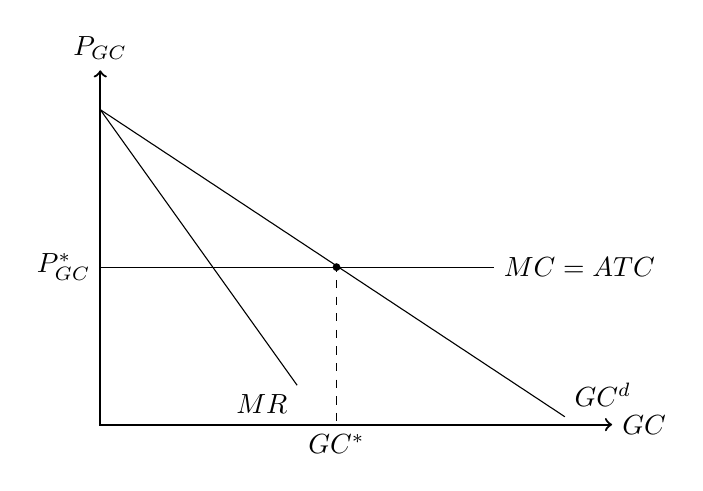
\begin{tikzpicture}
\tikzset{
	dot/.style={circle,inner sep=1pt,fill,name=#1},
}
% grid 
%\draw[step=1cm,gray,very thin] (-1.9,-1.9) grid (5.9,5.9);

% Draw axes
\draw [<->,thick] (0,4.5) node (yaxis) [above]{$P_{GC}$}
|- (6.5,0) node (xaxis) [right] {$GC$};

\draw (0,4)--(5.9,.1) node[above right, black]{$GC^d$};
\draw (0,4)--(2.5,.5) node[below left, black]{$MR$};

\draw (0,2)--(5,2) node[anchor=west, black]{$MC=ATC$};

\coordinate (opt0) at (3,2);

\draw[dashed] (yaxis |- opt0) node[left] {$P_{GC}^*$}
-| (xaxis -| opt0) node[below] {$GC^*$};
\node[dot=opt0] at (opt0) {};
\end{tikzpicture}

\end{standaloneframe}
\end{document}